%!TEX root = thesis.tex

\chapter{Anforderungen}
\label{chapter-analyse}

Um die relevanten Anforderungen, die Einfluss auf die Entwicklung und die spätere Nutzung des
Reservierungstools nehmen, identifizieren und einzuordnen zu können wurde eine Analyse nach dem
menschenzentrierten Gestaltungsprozess durchgeführt, um unter anderem Benutzende, Aufgaben und
Kontext des Projektes genauer zu verstehen. Nach einer Ausführung der Datenquellen
(\ref{section:daten}) wurden zunächst zwei Benutzergruppen (Verleihende und Ausleihende) mittels
einer Benutzeranalyse (\ref{section:benutzer}) unter der zu Hilfenahme der durchgeführten Interviews
klassifiziert und eingegrenzt. Daraufhin wurden die Probleme und Herausforderungen des aktuellen
Vorgehens und den unterschiedlichen Ausleihprozessen (\ref{section:iststand}) geschildert.
Anschließend wurden die Aufgaben, die Verleihende und Ausleihende mithilfe der Anwendung bewältigen
möchten, diskutiert (\ref{section:aufgaben}) sowie der organisatorische und zeitlich-räumliche
Kontext des Verleihens und Ausleihens am \ac{imis} (\ref{section:kontext}) untersucht. Aufbauend auf
den Resultaten der vorangestellten Untersuchungen wurden die objektiven Anforderungen an den SnipeIT
Companion formalisiert (\ref{section:anforderung}).

\section{Datenquellen}
\label{section:daten}
\todo[]{Literaturrechereche}
Im Rahmen der Analyse wurden Stakeholder-Interviews durchgeführt und ein vergleichbares Projekt
konnte im Rahmen eines Interviews als weitere Quelle genutzt werden. Die Befragten wurden durch ein
semi-strukturiertes Interview geführt. Im Vorfeld wurde dafür ein Interviewleitfaden entwickelt
(Anhang Verlinken). Es wurde eine Unterteilung in Verleihende und Ausleihende von Assets vorgenommen
(genauere Definition der Benutzergruppen in \ref{section:benutzer}). Bei den Teilnehmenden handelt
es sich um Mitarbeitende, welche am \ac{imis} tätig sind und Studierende der Medieninformatik an der
Universität zu Lübeck. In \ref{table:v} ist der jeweilige (Haupt-)Zuständigkeitsbereich der
Verleihenden aufgeführt. Die Verleihenden der Assets können gleichzeitig die Position eines
Ausleihenden einnehmen. Die Rollen der Ausleihend befragten umfassen sowohl Bachelorstudent als auch
Masterstudenten, diese sind in \ref{table:a} dargestellt. Die IDs der Teilnehmenden werden als
Verweise in den folgenden Abschnitten verwendet\footnote{die mit * gekennzeichneten Personen wurden
gemeinsam interviewt}. Des Weiteren wurde mithilfe des \ac{ati} das technische Interesse und
Verständnis der Teilnehmenden festgestellt, sodass das Reservierungstools entsprechend an die
Benutzergruppen angepasst werden kann \cite{attig_assessing_2017}.


\todo[]{Brauche ich das Alter?}
\begin{table}[h]
        \centering
        \caption{Teilnehmende der Interviews, Verleihende}
        \begin{tabular}{lll}
                \arrayrulecolor{maincolor}\hline
                \sffamily\color{maincolor}ID & \sffamily\color{maincolor}Alter &
                \sffamily\color{maincolor}Zuständigkeitsbereich \\
                \arrayrulecolor{maincolor}\hline
                V1                           & 25 - 35 J.                      & Keine direkte
                Zuständigkeit, Zugänge zu verschiedenen Laboren    \\
                V2                           & 25 - 35 J.                      & Multimedialabor \\
                V3                           & 25 - 35 J.                      & VR-Labor \\
                V4                           & 40 - 59 J.                      & Administratives
                Personal                                         \\
                V5                           & 25 - 35 J.                      & Innovationslabor \\
                \arrayrulecolor{maincolor}\hline
        \end{tabular}
        \label{table:v}
\end{table}

\begin{table}[h]
        \centering
        \caption{Teilnehmende der Interviews, Ausleihende}
        \begin{tabular}{ll}
                \arrayrulecolor{maincolor}\hline
                \sffamily\color{maincolor}ID & \sffamily\color{maincolor}Rolle \\
                \arrayrulecolor{maincolor}\hline
                A1                           & Bachelorstudentin, Hilfswissenschaftlerin \\
                A2                           & Bachelorstudent \\
                A3                           & Masterstudent, Hilfswissenschaftler \\
                A4*                          & Bachelorstudentin \\
                A5*                          & Bachelorstudentin \\
                A6                           & Masterstudentin \\
                \arrayrulecolor{maincolor}\hline
        \end{tabular}
        \label{table:a}
\end{table}

\section{Benutzeranalyse}
\label{section:benutzer}
Um eine zielgruppengerecht Gestaltung des SnipeIT Companion voraussetzten zu können, werden in
diesem Abschnitt die Benutzergruppen des Reservierungstools eruiert und näher untersucht.
Resultierend aus den Stakeholder-Interviews wurden zwei Benutzergruppen, zu denen Verleihende sowie
Ausleihende eines Assets gehören, für das System erarbeitet. Die Zielgruppe beschränkt sich im
Rahmen dieser Arbeit auf Mitarbeitenden des \ac{imis} sowie  Studierenden der Medieninformatik an
der Universität zu Lübeck.

Aus den Interviews (\ref{section:daten}) konnte entnommen werden, dass beide Benutzergruppen täglich
ein Smartphone, Tablet, Laptop oder Desktop PC nutzen und somit ein grundlegendes technisches
Verständnis vorausgesetzt werden kann. Diese Behauptung konnte mit den Ergebnissen der
\ac{ati}-Skala bestärkt werden (\ref{table:ati}). 

\begin{table}[h]
        \centering
        \caption{Werte der \ac{ati}-Skala}
        \begin{tabular}{lccc}
                \arrayrulecolor{maincolor}\hline
                \sffamily\color{maincolor}Benutzergruppe & \sffamily\color{maincolor}Mittelwert
                $(M)$& \sffamily\color{maincolor}Standardabweichung $(SD)$ &
                \sffamily\color{maincolor}Teilnehmende $(N)$ \\
                \arrayrulecolor{maincolor}\hline
                Verleihende & 5,00                                 & 0,58 & 3\\
                Ausleihende & 5,13                                 & 0,48 & 6\\
                \arrayrulecolor{maincolor}\hline
        \end{tabular}
        \label{table:ati}
\end{table}

%Mitarbeitende, sowie administratives Personal des \ac{imis}, welche verantwortlich für die Ausgabe
%von Assets sind, werden im folgenden als Verleihende bezeichnet (\ref{table:v}).
\subsection{Verleihende}
Mit $N=3$ und einem durchschnittlichen Alter von XX, lag der Wert der \ac{ati}-Skala, aufseiten der
Verleihenden, bei $M=5,00$ mit einer $SD=0,58$, dies weist auf eine geringe $SD$ hin und den
Nutzenden kann eine hohe Technikaffinität vorausgesetzt werden.

Verleihende umfassen ausschließlich Mitarbeitende, sowie administratives Personal des \ac{imis},
welche verantwortlich für die Ausgabe von Assets sind (\ref{table:v}). Verleihende sind in der Lage,
einzelne Assets herauszugeben. Allerdings haben nicht alle Verleihende auf alle Assets den gleichen
Zugriff, da dies von Forschungsgruppe zu Forschungsgruppe unterschiedlich ist. Zudem liegen in den
Forschungsgruppen unterschiedliche Vorgänge vor (genauere Unterschiede zu den Vorgängen in
\ref{section:iststand}). Folglich können Verleihende der Assets gleichzeitig die Position der
Ausleihenden einnehmen.

\subsection{Ausleihende}

Mit $N=6$ und einem durchschnittlichen Alter von XX, lag der Wert der \ac{ati}-Skala, aufseiten der
Ausleihenden, bei $M=5,13$ mit einer $SD=0,48$, dies weist auf eine geringe $SD$ hin und den
Nutzenden kann eine hohe Technikaffinität vorausgesetzt werden.

\todo[]{Was schreibe ich da noch groß zu?}
Bei den Ausleihenden handelt es sich insbesondere um Studierende, welche keinen direkten Zugang zu
den Assets haben (\ref{table:a}). Ausleihende suchen Mitarbeitende aktiv auf oder kontaktieren jene,
um Informationen über ausleihbare Assets zu erhalten. Wie bereits geschildert, können durch die
Forschungsgruppen auch Mitarbeitende, also Verleihende zu Ausleihenden werden, wobei für dergleichen
häufig ein anderer Ausleihprozess als für Studierende vorliegt (\ref{section:iststand}). 

\section{Problemanalyse}
\label{section:iststand}
        
Um die Relevanz des Verleihens am \ac{imis} sowie die Prozesse und damit einhergehenden
Problematiken besser nachvollziehen zu können, wurde eine Problemanalyse auf Basis der Interviews
getroffen. Der Übersichtlichkeit wegen werden im Folgenden Probleme, welche Verleihende und
Ausleihende betreffen thematisiert. Daraufhin werden Probleme der einzelnen Benutzergruppen näher
erläutert.

\subsection{Probleme: Allgemein}
\label{section:probleme-allgemein}
Eines der größten Probleme im derzeitigen Ablauf ist das nicht vorhanden sein, einer öffentlichen
Liste für Studieren, über die ausleihbare Assets eingesehen werden können. Auch aufseiten der
Verleihenden, also unter den \ac{wimi} ist keine vollständige interne Übersicht vorhanden (V,A).
Dies führt dazu, dass durch nicht wissen wenig Assets ausgeliehen werden können (alle). Durch die
verschiedenen Forschungsgruppen am \ac{imis} und die damit verbundenen Labore gibt es verschiedene
Ansprechpartner:innen für die jeweiligen Assets in den Laboren. Die Zuständigkeit dieser
Ansprechpartner:innen ist jedoch nicht ausreichend ersichtlich, sodass es häufig zu weiterverweisen,
an andere Ansprechpartner:innen kommt, wobei auch hier unter \ac{wimi} nicht immer klare
Ansprechpartner:innen ersichtlich sind (V1,V3, V4, A1, A2, A3). 

Studierende, welche als \ac{hiwi} am \ac{imis} angestellt sind, haben beim Ausleihen häufig einen
Vertrauensvorschuss, sodass bei Kurzem Verleihen und Tätigkeiten im Gebäude, Assets verliehen oder
entnommen werden, ohne dies zu Vermerken. Dies gilt auch für \ac{wimi} (A1, V1, V2).

Beim Verleihen von Assets kommt es häufig vor, dass insbesondere Studierende, ohne Wissen ein Asset
ausleihen wollen. Aufseiten der Verleihenden herrscht hier ein Ungleichgewicht, während einige auf
die Selbstaneignung und Google verweisen, ist es anderen wichtig, den Use Case der Nutzung zu
verstehen und die damit verbundenen Einstellungen der Assets sowie weiteres Zubehör zu empfehlen
(V1, V2, V4, V5, A3, A6). 

\todo[inline]{Sollten Assets beschädigt werden gibt es kein Verzeichnis für Gebrauchsspuren, ..
Technisches Gerät seine Macken hat auch keine Kenntnisse... (A1, V1).}

\subsection{Probleme: Verleihende}
Eine zentrale Schwachstelle des aktuellen Prozesses sind die uneinheitlichen Prozesse. Das Ausleihen
von Assets wird von Forschungsgruppe zu Forschungsgruppe unterschiedliche gehandhabt, bzw. innerhalb
der Forschungsgruppe liegen auch Unterschiede im Prozess vor (V1, V2,V3). Wie bereits in den
Allgemeinen Problemen (\ref{section:probleme-allgemein}) geschildert ist es einigen Verleihenden
wichtig, dass Ausleihende über die Assets Bescheid wissen und der Use Case detailliert besprochen
und erläutert wird, für wiederum andere ist die Vermittlung dieses Wissens nicht von Bedeutung
(V1,V2,V3,V4) (siehe Probleme: Ausleihende).

Um ein Asset ausleihen zu können, müssen Ausleihende auf einem Formular unterschreiben, in anderen
Fällen wird auf irgendeinem Zettel unterschrieben (V1, V2, V3, V4), dies führt zu einer
Zettelwirtschaft (V4, V5). Wiederum wird durch das Vertrauen am \ac{imis} und bei kurzen Dauern
nicht dokumentiert, wer oder wie lange das Gerät genutzt wird (V1, V2). Die Mitarbeitende, welche
von anderen Forschungsgruppen ein Asset ausleihen möchten, haben häufig einen anderen Ausleihprozess
als Studierende, da der Vertrauens- und Bekanntheitsgrad ein anderer ist (V1,V2,V3). Durch die
mangelnde und uneinsichtige Dokumentation des Ausleihens kann ein spontanes Planen erschwert werden
(V1, V2, V3, ...).

Da auch eine interne Übersicht der Verfügbaren Assets für Verleihende nicht vorhanden ist, kommt es
durch Unwissenheit zu Doppelbeschaffung (V1, V2, V3). Folglich kann es zu Anschaffungen kommen,
welche mit dem vorhanden Assets nicht kompatible sind (V2,V3). Eine Schwachstelle liegt im
Beschaffen von Assets, ohne dass diese vermerkt werden. Dies führt dazu, dass Assets in einzelnen
Büros liegt oder vergessen werden, obwohl diese für Laufende Studien o. Ä. sinnvoll sein können
(V3). Angeschaffte Asset werden nach zwei Jahre wieder gefunden (V1, V2, V3).

\todo[inline]{Keine Wartung oder Person, die sich so richtig verantwortlich fühlt, bzw. die Person,
die es gekauft hat ist zuständig,... Akku leer, ... nicht vernünftig zurückgelegt (V1, V2, V5)}

\subsection{Probleme: Ausleihende}
% Verantwortlichkeiten unklar (für Studierende) (A1, A2, A5)
Für Studierende ist das ausleihen insofern schwer, als das höchstens über Flurfunk, Videoworkshop
oder vereinzelnd Übungen über einzelne Assets berichtet wird (alle As). Der Vorgang, per E-Mail sei
für einige Studierende entspannt, trotzdem erschwert es das ausleihen, wenn nicht Bescheid gegeben
wird was Ausleihbar ist (A4, A5). Wiederum andere empfinden das E-Mail schreiben als störend,
insbesondere, wenn bewusst ist wie viel \ac{wimi} zu tun haben und die Antwortzeit entsprechend hoch
ist. Daher ist spontanes planen unzuverlässig (A1, A6). Spontanes nachfragen nach Assets ist
aufseiten der Studierenden weniger zu sehen. Hier wird vorher eine Mail an einen \ac{wimi}, in den
meisten Fällen an die verantwortlichen Übungsleiter oder die Studiengangkoordination, geschrieben,
weil das Risiko zu hoch sei, das Asset nicht verfügbar sind (A3). Stark bemängelt wird jedoch, dass
es keine Garantie gibt, dass etwas zum gewünschten Zeitpunkt ausleihbar ist (A1, A3) und noch dazu
kein schnelles Herankommen, ermöglicht werden kann (A3). Außerdem wird kritisiert, dass das
nachfragen als nervig wahrgenommen wird, weil \ac{wimi}, für simple Fragen, die eine Liste der
Assets beantworten würde, aus der Arbeit gerissen werden (A6). Dazu kommt, dass Ausleihende nicht
genau wissen, um was für ein Gerät es genau handelt, so kann es zu Kompatibilitätsfehlern kommen,
weil die Auskunft fehlt und eine Selbstaneignung vorausgesetzt wird (A3). Dies führt dazu, das
Projekt konnte nicht mit dem Asset umgesetzt werden konnten (A3). Folglich können Ausleihende nur
bedingt mit den Geräten umgehen.


\section{Aufgabenanalyse}
\label{section:aufgaben}
Durch die Aufgaben, welche Verleihende und Ausleihende im Ausleihprozess durchlaufen, konnte
resultierend auf Basis der Interviews (\ref{section:daten}) Aufgaben erarbeitet werden, welche von
dem Reservierungstools übernommen oder unterstützt werden können. Die Aufgaben wurden anhand des
Ausleihprozesses in drei Bereiche eingeordnet. Im ersten Bereich handelt es sich um die
Vorbereitung, welche zum Ausleihen eines Assets getroffen werden müssen. Darauffolgend werden die
Aufgaben der Ausgabe definiert. Der dritte Bereich umfasst die Rückgabe der Assets. Ergänzend zu den
zuvor genannten Bereichen wurden Aufgaben für die Wartung der Assets dargestellt.

% 1. Überschrift ausgeführt 2. wer und besonderheiten (Zielgruppe) 3. Rahmenbediungen 4. Details

% Aufgabe im Bereich der Vorbereitung
\subsection{Aufgaben im Bereich der Vorbereitung}
Um ein Asset ausleihen zu können, müssen bestimmte Vorbereitungen getroffen werden, diese werden im
Folgenden näher erläutert.
\subsubsection{Ag-Vt-1 | Verfügbarkeit anfragen}
\label{subsubsection:Ag-Vt-1}
Um ein Asset ausleihen zu können, muss eine Anfrage an die verantwortlichen gesendet werden, dies
geschieht meist per E-Mail. Ausleihende fragen, aufgrund des mangelnden Wissen, nach einem direkten
Asset, welches über bspw. den Flurfunk an diese gelang. Wie bereits in der Problemanalyse geschildert
(\ref{section:probleme-allgemein}) gibt es keine Übersicht, über ausleihbare Assets. Dies zeigt die
Dringlichkeit des SnipeIT Companion für eine besser Vorbereitung. So können Ausleihende mit mehr
Wissen eine Anfrage zum Ausleihen stellen. 
\subsubsection{Ag-Vt-2 | Verfügbarkeit einsehen}
\label{subsubsection:Ag-Vt-2}
Um ein Asset ausleihen zu können ist es sowohl für Verleihende als auch Ausleihende von Bedeutung,
ob Assets Verfügbar sind. Verleihende überprüfen, ob das angefragte Asset im Schrank vorhanden ist.
Hierbei ist zu berücksichtigen, dass keine langfristige Planung in die Zukunft nicht gewährleistet
werden kann. Dies kann jedoch mit dem SnipeIT Companion mittels eines Kalenders und einer
Reservierungsfunktion ermöglicht werden.
\subsubsection{Ag-Vt-3 | Reservierungen von Assets}
\label{subsubsection:Ag-Vt-3}
Wie in \nameref{subsubsection:Ag-Vt-2} bereits geschildert, kann eine langfristige Planung in die
Zukunft nicht gewährleistet werden. Liegt eine Anfrage in die Zukunft vor, wird diese mittels eines
Klebezettels am gewünschten Asset vermerkt. Am Ende muss gehofft werden, dass die Notiz von
\ac{wimi} berücksichtigt wird und das Asset zum gewünschten Zeitraum verfügbar ist.
\subsubsection{Ag-Vt-4 | Beratungsgespräch }
\label{subsubsection:Ag-Vt-4}
Die zuvor erhaltene Anfrage aus \nameref{subsubsection:Ag-Vt-1} wird von Verleihenden verarbeitet,
wobei in den meisten Fällen der Use Case des ausleihens eruiert wird, um den Ausleihenden Tipps zu
vermitteln. Um den Ausleihprozess für Verleihende zu erleichtern, kann der vorangestellt Use Case
mittels eines Dialogs ermöglicht werde. So können aufbauend auf dem Dialog, direkt Vorschläge an
Ausleihende gegeben werden.


% Aufgabe der Ausgabe 
\subsection{Aufgaben im Bereich der Ausgabe}
Im nächsten Abschnitt werden alle zentralen Aufgaben aufgeführt, welche für die Übergabe von
Verleihnden zu Ausleihnden umfasst.
\subsubsection{Ag-Au-1 | Abholung}
Aushleihende holen die Assets am \ac{imis} ab. Verleihende schaffen hierfür Zugriff zum Labor oder
Schrank. 
\subsubsection{Ag-Au-2 | Nutzung von Assets erläutern}
Ausleihende wissen vorher häufig nicht genau um was für ein Gerät es sich genau handelt, so kann es
zu Kompatiblitätsfehlern kommen und das Asset ist für den ursprünglichen Gebrauch nicht nutzbar. Daher
kann in einigen Fällen eine kurze Erklärung zur Nutzung für den Ausleihenden hilfreich sein. Im
besten Fall, ist eine Übersicht mit Informationen wie: Name, Seriennummer, usw. sowie der dazugehörigen
Anleitung bereits vor dem Ausleihprozesse verfügbar, sodass Ausleihende sich im Vorhinein selbständig
besser informieren können.
\subsubsection{Ag-Au-3 | Formular unterschreiben}
In einigen Fällen werden die ausgeliehene Assets in einem Formular dokumentiert, welches von den
Ausleihenden unterzeichnet wird. Das Formular wird bis zur Rückgabe aufbewahrt. Durch die
unterschiedlichen Vorgänge ist diese Aufgabe nicht immer einheitlich.

% Aufgaben der Rückgabe
\subsection{Aufgaben im Bereich der Rückgabe}
Die Nachfolgenden Aufgaben umfassen die Rückgabe der ausgeliehenen Assets. 

\subsubsection{Ag-Rg-1 | Rückgabe}
Für die Rückgabe der ausgeliehenen Assets wird auf dem Formular dokumentiert wann, was zurückgegeben
wurde. Die Rückgabe wird meist während der Abholung besprochen oder per E-Mail. In den Fällen, in
den kein Formular ausgefüllt wurde, wird der Klebezettel mit der Unterschrift entsorgt und in wieder
anderen Fällen werden die Assets direkt in die Schränke und Räume zurückgebracht.
\subsubsection{Ag-Rg-2 | Überprüfung}
Für einige Verleihenden fällt die Überprüfung der Assets nach einer Rückgabe an. Hier wird geschaut,
dass bspw. SD Karten gelehrt wurden und Akkus geladen. Außerdem können Einstellungen an den Assets
zurückgesetzt werden. 
% Aufgaben der Wartung
\subsection{Aufgaben im Bereich der Wartung}
\label{subsec:wartung}
Im Folgenden werden Aufgaben, welche für Verleihende auf Administariver Ebene von Bedeutung sind
näher erläutert. 

\subsubsection{Ag-Wt-1 | Pflege von Assets}
\label{subsubsection:Ag-Wt-1}
\todo{Findet das Überhaupt statt?}
Assets, die längere Zeit nicht genutzt werden, müssen von Verleihenden gewartet werde. Dies Gerät in
manchen Fällen eher in Vergessenheit. 

\subsubsection{Ag-Wt-2 | Neuanschaffung}
\label{subsubsection:Ag-Wt-2}
Bei Neuanschaffung, keinen Überblick über die Erneuerungen, ...



\section{Kontextanalyse}
\label{section:kontext}

Für die Ermittlung der Nutzungsumgebung, in der das System verwendet werden soll, wurde eine
Kontextanalyse, basierend auf den vorangehenden Analysen sowie den Interviews durchgeführt. Zunächst
wurde der organisatorische Kontext, des Systems festgehalten. Anschließen werden der
zeitlich-räumliche sowie technische Kontext eruiert \cite{herczeg_einfuhrung_2009}.

\subsection{Organisatorischer Kontext}
Unter Berücksichtigung von sozialen Strukturen kann maßgeblich die Qualität des Systems positiv
beeinflusst werden \cite{herczeg_einfuhrung_2009}. Aus diesem Grund wurden die Strukturen untersucht
und in formelle und informelle organisatorische Strukturen unterteilt.

\subsubsection{Formelle Organisation}
Innerhalb des Universitäts-Kontextes gibt es aus formaler Sicht eine überwiegend flache Hierarchie
zwischen Studierenden und Mitarbeitenden, wobei zwischen Hilfswissenschaftlern:innen,
wissenschaftlichen Mitarbeitenden sowie Professor:innen unterschieden werden kann. Diese Gruppen
weisen teilweise verschiedene Zugriffe auf bestimmte Labor und Schränke, welche die Assets
beinhaltet auf.

Um die \nameref{subsec:wartung} berücksichtigen zu können sollten Verleihende einen administrativen
Zugang zum System erhalten, um neue Assets eintragen zu können (\nameref{subsubsection:Ag-Wt-2}). Des Weiteren sollte so
ein Überblick über Updates ö. Ä. gegeben werden können (\nameref{subsubsection:Ag-Wt-1}). 

\subsubsection{Informelle Organisation}
??
\subsection{Zeitlich-Räumlicher Kontext}
\label{section:zeit}
Der zeitlich-räumliche Kontext sollte sowohl aus Sicht der Verleihenden als auch aus Sicht der
Ausleihenden analysiert werden, da die Anwendung einen einheitlichen Ausleihprozess schaffen soll. 

\subsubsection{Verleihende}
Mitarbeitende halten sich entweder in ihren Büros oder an einem anderen Ort auf, daher werden bei
der Analyse des zeitlich-räumlichen Kontextes beide Fälle betrachtet.

Befinden sich Mitarbeitende im Büro, arbeiten diese an einem Desktop-Arbeitsplatz. Der Computer ist
dabei die meiste Zeit eingeschaltet, daher wäre ein System in beispielsweise Form einer Web-App
sinnvoll (V1,V5). Wenn Mitarbeitende das Büro verlassen, um ein Asset zu Verleihen, können sich
\ac{wimi} in verschiedenen Laboren aufhalten/befinden. Da der Ort der Nutzung variiert, liegt ein
mobiler Nutzungskontext vor, welcher beispielsweise durch die Nutzung einer Web-App auf dem
Smartphone ermöglicht werden kann (V1, V2, V3, V5). Die Bedienung der Anwendung sollte
niedrigschwellig sein, da Mitarbeitende häufig nicht viel Zeit für die Bedienung haben oder
investieren möchten. Das System sollte einen pragmatischen Zweck erfüllen und kein zu großes Konzept
umfasse, sodass womöglich neue Anläufe dazu kommen und die Arbeit zweckmäßig eher erhört, als
verringert (V2).

\subsubsection{Ausleihende}
Studierende arbeiten sowohl von Zuhause aus, als auch in der Bib , ... 

Da das Buchen von Assets auch in spontanen Momenten gefragt ist, variiert die Nutzung des Systems
auch hier. Daher liegt ein mobiler Nutzungskontext vor, welcher beispielsweise durch die Nutzung
einer Web-App auf dem Smartphone ermöglicht werden kann (A1, A3, A6).

\subsection{Technischer Kontext}
Eingliedern?


\section{Formalisierte Anforderungen}
\label{section:anforderung}
%Wie eingangs er-wähnt, definieren die Anforderungen, was das System zu leisten hat, während die
%Funktionalitä-ten definieren, wie das System diese gewährleistet.

Im Folgenden werden systematisch formalisierte Anforderungen präsentiert, welche die Ergebnisse der
Analysen abschließend zusammenfassen. Es werden zunächst die Visionen und Ziele
(\ref{section:visionziel}) definiert, des Weiteren werden die Rahmenbedingungen
(\ref{section:rahmen}) und der Kontext des Systems (\ref{section:kontextueberblick}) dargestellt.
Darauf aufbauend wird eine funktionale Anforderung erstellt (\ref{section:funktionale}). Abschließen
werden die Qualitätsanforderungen formuliert (\ref{section:qualität}).


\subsection{Vision und Ziele}
\label{section:visionziel}
Zunächst werden die Visionen und Ziele des Systems konkretisiert, an denen sich die Anforderungen
auf Zielgerichtetheit überprüfen lassen \cite{balzert2009}. Diese setzen sich aus der Analyse der
Benutzenden sowie Aufgaben und des Kontextes zusammen. Zunächst werden die Visionen für die
Zukunft realitätsnah festgelegt.

\begin{center}
        \renewcommand{\arraystretch}{1.5}
        \begin{tabular}{p{0.1\textwidth}p{0.8\textwidth}}
                \hline
                \textbf{/V10/} & Der SnipeIT Companion unterstützt Ausleihende effizient mit
                individuellen und anwendungsspezifischen Assetvorschlägen.\\
                \textbf{/V20/} & Der Ausleihprozess von Assets am \ac{imis} verläuft einheitlich.\\
                \textbf{/V30/} & Ausleihbare Assets des \ac{imis} sind (allen) bekannt und werden sowohl von
                Studierenden, als auch von Mitarbeitenden genutzt.\\
                \textbf{/V70/} & Die Planung und Kommunikation zwischen Studierenden sowie
                Forschungsgruppen untereinander verläuft Reibungsloser.\\
                \textbf{/V71/} & Es kommt zu keinen unbeabsichtigten Doppelbeschaffungen.\\
                \textbf{/V80/} & Verleihende fühlen sich durch den SnipeIT Companion unterstützt.\\
                \hline
        \end{tabular}
\end{center}

Basierend auf diese Visionen lassen sich die Ziele formulieren, welche die Visionen
operationalisieren. Diese folgen dabei den standardisierten Regeln zur Formulierung von Zielen
\cite{pohl_requirements_2008}.


\begin{center}
        \renewcommand{\arraystretch}{1.5}
        \begin{tabular}{p{0.1\textwidth}p{0.8\textwidth}}
                \hline
                \textbf{/Z10/} & Ausleihende eines Assets erhalten zielgerichtete und aktuelle
                Informationen zum Asset. \\
                \textbf{/Z20/} & Ausleihende sind jederzeit in der Lage .??? \\
                \textbf{/Z30/} & Ausleihende sollen standortunabhängig in der Lage sein, die
                Verfügbarkeit von Assets einsehen zu können und diese zu buchen, (damit die
                 direkt und ohne Umwege für den Ausleihenden effizient innerhalb einer
                Anwendung erledigt werden kann). \\
                \textbf{/Z40/} & Ausleihende sollen jederzeit in der Lage sein, in der Ausführung des
                SnipeIT Companion Unterstützung zu bekommen, damit deren Lernprozess gefördert
                und so Assets häufiger genutzt werden. (Bezug, was lernen) \\
                \textbf{/Z50/} & Ausleihende sollen jederzeit in der Lage sein, sich über Assets zu
                informieren, damit diese initiale Nutzungsbarrieren überwinden können und sich auf
                die Praxis des Assets vorbereiten können.\\
                 \textbf{/Z60/} & Ausleihende
                verwenden ein gebrauchstaugliches, niedrigschwelliges Interface zum Ausleihen von
                Assets. \\
                \textbf{/Z70/} & Das System soll Informationen zugänglich präsentieren.\\
                \textbf{/Z80/} & Verleihende sollen jederzeit in der Lage sein, vom System
                gesammelte Daten übersichtlich und strukturiert einzusehen (Wartung).\\
                \hline
        \end{tabular}
\end{center}

\subsection{Rahmenbedingungen}
\label{section:rahmen}
Die Randbedingungen legen organisatorische und technische Restriktionen für das System oder den
Entwicklungsprozess fest \cite{balzert2009}. Die Bedingungen wurden aus der Benutzer- und
Kontextanalyse abgeleitet.

\begin{center}
        \renewcommand{\arraystretch}{1.5}
        \begin{tabular}{p{0.1\textwidth}p{0.8\textwidth}}
                \hline
                \textbf{/R10/} & Das System ist eine Web-Anwendung. \\
                \textbf{/R20/} & Die Zielgruppe sind Mitarbeitende des IMIS und Studierende. \\
                \textbf{/R30/} & Die Zielgruppe teilt sich in zwei Nutzergruppen: die Verleihenden
                und Ausleihende von Assets. Die Definitionen der Nutzergruppen sind in Kapitel
                (\secref{section:benutzer}) zu finden. \\
                \textbf{/R40/} & Das System wird von Verleihenden sowohl im mobilen als auch im
                ...Kontext genutzt. \\
                \textbf{/R50/} & Die eingesetzte Software auf der Zielmaschine ist clientseitig ein
                Webbrowser. Die marktführenden Webbrowser müssen unterstützt werden: Chrome,
                Firefox, Safari \cite{noauthor_browser_nodate}. \\
                \hline
        \end{tabular}
\end{center}

\subsection{Kontext und Überblick}
\label{section:kontextueberblick}
Ein System ist in einer technischen Umgebung eingebettet \cite{balzert2009}. Es wurde im folgenden
Bezug auf das aktuelle Vorgehen mithilfe der Problemanalyse geschlossen.

\begin{center}
        \renewcommand{\arraystretch}{1.5}
        \begin{tabular}{p{0.1\textwidth}p{0.8\textwidth}}
                \hline
                \textbf{/K10/} & Das aktuelle Vorgehen umfasst keine Liste für Verleihende und
                Ausleihende. \\
                \textbf{/K20/} & Es kommmt zu Doppelbeschaffungen. \\
                \textbf{/K30/} & Es existieren von Forschungsgruppe zu Forschungsgruppe
                unterschiedliche Ausleihprozesse. \\
                \hline
        \end{tabular}
\end{center}

\subsection{Funktionale Anforderungen}
\label{section:funktionale}
Im Folgenden werden die Kernfunktionalitäten des Systems aufgeführt \cite{balzert2009}. Diese
ergeben sich aus der Aufgabenanalyse (\ref{section:aufgaben}). Um die Anforderungen mit einer
eindeutigen Semantik zu formulieren, wurde eine Anforderungsschablone (\ref{fig:schablone})
verwendet, um natürlichsprachliche Anforderungen zu definieren \cite{balzert2009}.

\begin{figure}[h]
        \centering
        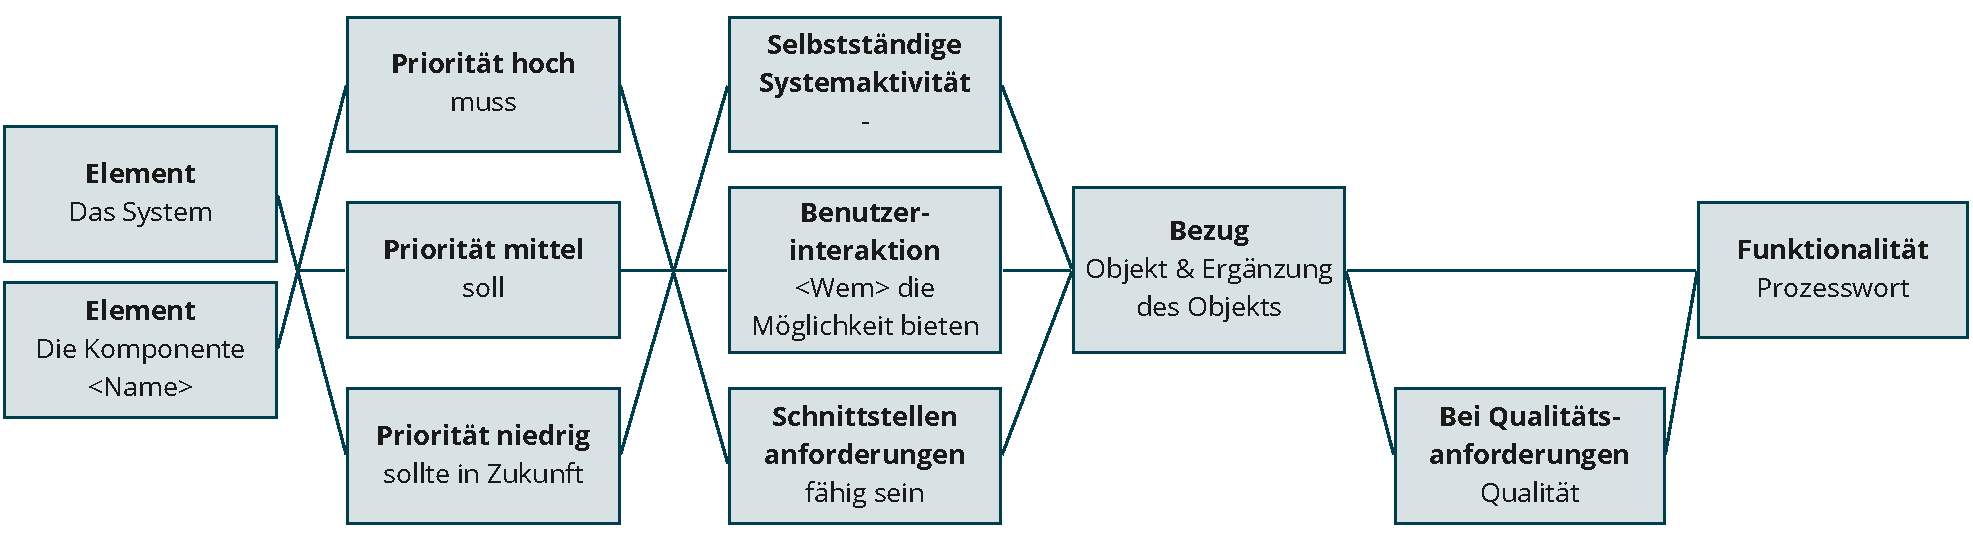
\includegraphics[scale=0.45]{Bilder/anforderungsschablone.pdf}
        \label{fig:schablone}
        \caption[Anforderungsschablone]{Anforderungsschablone \cite{balzert2009}}
\end{figure}


\begin{center}
        \renewcommand{\arraystretch}{1.5}
        \begin{tabular}{p{0.1\textwidth}p{0.8\textwidth}}
                \hline
                \textbf{/F10/}  & Das System \textit{muss} Verleihenden und Ausleihenden die
                Möglichkeit bieten, eine Übersicht der Assets jederzeit einsehen zu können (A). \\
                \textbf{/F20/}  & Das System \textit{muss} XX die Möglichkeit bieten,  . \\
                \textbf{/F30/}  & Das System \textit{muss} XX die Möglichkeit bieten,  (A). \\
                \textbf{/F40/}  & Das System \textit{muss} XX relevante Informationen anzeigen, (A).
                \\
                \textbf{/F50/}  & Das System \textit{muss} XX die Möglichkeit geben,. \\
                \textbf{/F60/}  & Das System \textit{soll} die Möglichkeit bieten, individuelle und
                personalisierte Inhalte zu visualisieren -> Checkliste (A). \\
                \textbf{/F70/}  & Das System \textit{soll} daran erinnern, die Ausgeliehenen Assets
                zurückzubringen oder zu verlängern oder abzuholen (A). \\
                \textbf{/F80/}  & Das System \textit{soll} XX die Möglichkeit bieten, . \\
                \textbf{/F90/}  & Das System \textit{sollte in Zukunft} . \\
                \textbf{/F100/} & Das System \textit{sollte in Zukunft} XX die Möglichkeit bieten,
                Informationen zu hinterlassen (A). \\
                \textbf{/F110/} & Das System \textit{sollte in Zukunft} . \\
                \hline
        \end{tabular}
\end{center}


\subsection{Qualitätsanforderungen}
\label{section:qualität}
Im letzten Schritt werden die nicht-funktionalen Anforderungen festgelegt, welche die qualitativen
oder quantitativen Eigenschaften eines Systems darstellen \cite{balzert2009}. Auch hier wird, falls
möglich, die Anforderungsschablone aus \ref{fig:schablone} verwendet.

\begin{center}
        \renewcommand{\arraystretch}{1.5}
        \begin{tabular}{p{0.1\textwidth}p{0.8\textwidth}}
                \hline
                \textbf{/Q10/} & Das System \textit{muss} den Grundsätzen der DIN EN ISO
                9241-110:2019-09 (Ergonomie der Mensch-System-Interaktion - Teil 110:
                Interaktionsprinzipien) folgen (\textit{DIN EN ISO 9241-110}, 2019). \\
                \textbf{/Q20/} & Das System \textit{muss} die definierten Nutzungsklassen aus
                \ref{section:benutzer} unterscheiden und die dazugehörigen Zugriffsrechte
                sicherstellen. \\
                \textbf{/Q30/} & Das System \textit{soll} modular strukturiert sein, damit Inhalte
                und Funktionalitäten effizient eingebunden werden können und das System einfach
                erweiterbar ist. \\
                \textbf{/Q40/} & Das System \textit{soll} beim Zugriff über das Internet eine
                gesicherte Übertragung (bspw. \ac{HTTPS}) ermöglichen. \\
                \textbf{/Q50/} & Das System \textit{soll} alle Benutzerinteraktionen in unter fünf
                Sekunden ausführen. \\
                \hline
        \end{tabular}
\end{center}
